\documentclass[12pt,letterpaper]{article}
\usepackage[margin=1in]{geometry}
\usepackage[T1]{fontenc}
\usepackage{mathptmx}          % Times (Times New Roman metric-compatible)
\usepackage{amsmath,amssymb}
\usepackage{graphicx}
\usepackage{booktabs,array,multirow}
\usepackage{xcolor}
\usepackage{enumitem}
\usepackage{etoolbox}
\usepackage[font=footnotesize,labelfont=normalfont,labelsep=period]{caption}
\usepackage{tikz}
\usetikzlibrary{arrows.meta,positioning,calc}
\usepackage{titlesec}
\usepackage{cite}
\usepackage{tocloft}
\usepackage[colorlinks=true,linkcolor=black,citecolor=black,urlcolor=black]{hyperref}

\newcommand{\Nsamples}{114{,}300}
\newcommand{\Nseg}{3810}
\newcommand{\Tdur}{3771.9}
\newcommand{\xmean}{431.7}
\newcommand{\xstd}{12.2}
\newcommand{\xmin}{257.1}
\newcommand{\xmax}{566.5}
\newcommand{\Nnan}{0}
\newcommand{\maxflat}{5}
\newcommand{\rulesRealNA}{3734}
\newcommand{\rulesRealNR}{76}
\newcommand{\rulesRealDA}{0}
\newcommand{\rulesRealDR}{0}
\newcommand{\Nrd}{4}
\newcommand{\trainRows}{11{,}208}
\newcommand{\trainNA}{9{,}066}
\newcommand{\trainNR}{618}
\newcommand{\trainDA}{1{,}428}
\newcommand{\trainDR}{96}
\newcommand{\nFeat}{70}
\newcommand{\rfRealNA}{3738}
\newcommand{\rfRealNR}{72}
\newcommand{\rfRealDA}{0}
\newcommand{\rfRealDR}{0}
\newcommand{\rfRealDefects}{0}
\newcommand{\rulesRealDefects}{0}
\newcommand{\realDiffSeg}{4}
\newcommand{\realAgree}{99.90}
\newcommand{\diffMaxDist}{1}
\newcommand{\diffAllNRtoNA}{1}
\newcommand{\hpFArf}{0}
\newcommand{\hpFAru}{6}
\newcommand{\hpOKrf}{17}
\newcommand{\hpOKru}{17}
\newcommand{\hpEvents}{17}
\newcommand{\hpRfNA}{3651}
\newcommand{\hpRuNA}{3635}
\newcommand{\hpRfNR}{70}
\newcommand{\hpRuNR}{74}
\newcommand{\hpRfDA}{87}
\newcommand{\hpRuDA}{99}
\newcommand{\hpRfDR}{2}
\newcommand{\hpRuDR}{2}
\newcommand{\hpTruthSeg}{89}
\newcommand{\hpPredRf}{89}
\newcommand{\hpHitRf}{88}
\newcommand{\hpExtraRf}{1}
\newcommand{\hpMissRf}{1}
\newcommand{\hpPredRu}{101}
\newcommand{\hpHitRu}{89}
\newcommand{\hpExtraRu}{12}
\newcommand{\hpMissRu}{0}
\newcommand{\hoN}{9205}
\newcommand{\hoRfAcc}{98.3}
\newcommand{\hoRfNA}{99.5}
\newcommand{\hoRfNR}{92.1}
\newcommand{\hoRfDA}{96.8}
\newcommand{\hoRfDR}{41.4}
\newcommand{\hoRuAcc}{92.3}
\newcommand{\hoRuNA}{94.3}
\newcommand{\hoRuNR}{70.5}
\newcommand{\hoRuDA}{91.6}
\newcommand{\hoRuDR}{43.7}
\newcommand{\hoFARf}{4}
\newcommand{\hoRfMV}{69/72}
\newcommand{\hoRfOL}{137/140}
\newcommand{\hoRfFDI}{40/40}
\newcommand{\hoFARu}{333}
\newcommand{\hoRuMV}{64/72}
\newcommand{\hoRuOL}{131/140}
\newcommand{\hoRuFDI}{38/40}
\newcommand{\hoEvents}{252}
\newcommand{\topFeatA}{ratio\_max@+2}
\newcommand{\topFeatB}{spike\_abs}


\newcommand{\ReportTitle}{Operational State and Data-Integrity Classification of PMU Measurements for Power System Oscillation Monitoring}
\newcommand{\ReportAuthor}{MD Mizgan Ali}
\newcommand{\ReportRoll}{123EE0257}
\newcommand{\ReportTitleA}{Operational State and Data-Integrity}
\newcommand{\ReportTitleB}{Classification of PMU Measurements}
\newcommand{\ReportTitleC}{for Power System Oscillation Monitoring}
\newcommand{\ReportDate}{October 2026}
\newcommand{\ReportSupervisor}{Prof.\ \textcolor{red}{[Supervisor Name]}}

% ---- IEEE-style headings, captions; 12 pt Times, 1.5 line spacing
\linespread{1.43}\selectfont
\setlength{\parskip}{0pt}\setlength{\parindent}{1.4em}
\renewcommand{\thesection}{\Roman{section}}
\renewcommand{\thesubsection}{\Alph{subsection}}
\titleformat{\section}{\centering\normalfont\normalsize\bfseries\scshape}{\thesection.}{0.5em}{}
\titleformat{\subsection}{\normalfont\normalsize\itshape}{\thesubsection.}{0.5em}{}
\titlespacing*{\section}{0pt}{1.0ex plus 0.3ex}{0.4ex}
\titlespacing*{\subsection}{0pt}{0.8ex plus 0.3ex}{0.3ex}
\renewcommand{\figurename}{Fig.}
\renewcommand{\tablename}{Table}
\renewcommand{\thetable}{\arabic{table}}
\captionsetup[table]{labelsep=period,justification=centering,position=below,skip=6pt}
\captionsetup[figure]{justification=justified,singlelinecheck=true}
\AtBeginEnvironment{figure}{\linespread{1}\selectfont}
\AtBeginEnvironment{table}{\linespread{1}\selectfont}
\setlist{itemsep=0pt,topsep=0pt,parsep=0pt}
\setlength{\textfloatsep}{8pt plus 2pt minus 2pt}
\setlength{\floatsep}{6pt plus 2pt minus 2pt}
\setlength{\intextsep}{6pt plus 2pt minus 2pt}
\renewcommand{\topfraction}{0.9}\renewcommand{\floatpagefraction}{0.8}
\renewcommand{\cftsecfont}{\bfseries}
\renewcommand{\cftsecpagefont}{\bfseries}
\renewcommand{\cftsecleader}{\hfill}
\renewcommand{\cftsubsecleader}{\cftdotfill{\cftdotsep}}
\renewcommand{\cftsecpresnum}{}
\setlength{\cftbeforesecskip}{1.1ex}
\setlength{\cftsecnumwidth}{2.6em}
\setlength{\cftsubsecindent}{2.6em}
\setlength{\cftsubsecnumwidth}{3.2em}
\renewcommand{\cfttoctitlefont}{\hfill\large\bfseries}
\renewcommand{\cftaftertoctitle}{\hfill}
\renewcommand{\thesubsection}{\thesection-\Alph{subsection}}
\newcommand{\code}[1]{\texttt{#1}}

\begin{document}
% =================================================================== TITLE PAGE
\begin{titlepage}\linespread{1.15}\selectfont
\centering
\vspace*{0.1in}

\includegraphics[width=1.7in]{nitr_logo.png}\par
\vspace{0.4in}
{\large Mid-Term Evaluation Report}\par
\vspace{0.15in}
on\par
\vspace{0.3in}
{\Large\bfseries Operational State and Data-Integrity Classification\par
of PMU Measurements for Power System\par
Oscillation Monitoring\par}
\vspace{0.45in}
{\itshape Department of Electrical Engineering}\par
\vspace{0.1in}
{\itshape National Institute of Technology, Rourkela}\par
\vspace{0.45in}
{\itshape Submitted by:}\par
\vspace{0.12in}
{\bfseries MD Mizgan Ali (123EE0257)}\par
\vspace{0.08in}
{\bfseries Sameer Shaik (123EE0047)}\par
\vspace{0.4in}
{\itshape Under the guidance of:}\par
\vspace{0.12in}
{\bfseries Prof.\ Shekha Rai}\par
\vfill
\begin{flushright}
\begin{minipage}{2.5in}\centering
\rule{2.5in}{0.5pt}\par
\vspace{0.6ex}
Signature of Supervisor
\end{minipage}
\end{flushright}
\end{titlepage}

\pagenumbering{roman}
\setcounter{page}{1}

% =================================================================== ABSTRACT
\begin{center}{\large\bfseries Abstract}\end{center}
\vspace{-0.5ex}
\noindent
Wide-area monitoring of power-system oscillations relies on phasor measurement unit (PMU) data, but the algorithms that estimate oscillation modes assume that the data are of good quality and that the type of excitation is known. This report presents the first two stages of a PMU-based mode-estimation workflow: (i)~classification of every one-second segment of a measured power signal into four \emph{operational states}---normal ambient (NA), normal ringdown (NR), degraded ambient (DA) and degraded ringdown (DR)---and (ii)~classification of the degraded segments into three \emph{integrity classes}---missing values (MV), outliers (OL) and false data injection (FDI).

Two classifiers are developed and compared. The first is a transparent rule-based classifier built on a short-term/long-term energy detector for ringdowns and three signal-integrity checks. The second is a pair of Random Forest classifiers that learn the decision thresholds from labelled examples. Because the measured record supplied for the project (\Nsamples{} samples, \Tdur{}\,s, four ringdown events) contains no faults, validation uses synthetic faults injected into a copy of the data with exactly known positions and types.

On the real record, both classifiers find only clean ambient and ringdown data and agree on \realAgree\,\% of the \Nseg{} segments. On a hand-placed set of \hpEvents{} injected faults both classifiers type every fault correctly, with \hpFAru{} (rules) and \hpFArf{} (Random Forest) false-alarm segments. On five randomly generated hold-out scenarios the Random Forest reaches a state accuracy of \hoRfAcc\,\% against \hoRuAcc\,\% for the rule-based classifier. The limitations of this validation, and the remaining stages of the workflow (data recovery, mode estimation and stability assessment), are discussed.

\clearpage
% =================================================================== CONTENTS
\begin{center}{\large\bfseries Contents}\end{center}
\vspace{2ex}
{\renewcommand{\contentsname}{}\setlength{\cftbeforetoctitleskip}{0pt}\setlength{\cftaftertoctitleskip}{0pt}\tableofcontents}
\clearpage
\pagenumbering{arabic}
\setcounter{page}{1}

\section{Introduction}
Electromechanical oscillations between generators are inherent in interconnected power systems, and their frequency and damping ratio indicate how close the system is to instability \cite{kundur2004}. PMUs provide synchronised, high-rate measurements from which these modes can be estimated continuously. Two kinds of data must be distinguished: \emph{ambient} data, produced by small random load variations, and \emph{ringdown} data, a decaying oscillation after a large disturbance. They need different estimators. Real PMU streams are also imperfect: samples go missing, isolated outliers appear, and data can be altered by a false data injection (FDI) attack \cite{liu2009}, which makes the estimated modes unreliable.

The project therefore builds a workflow that first classifies the data by operating condition and by integrity, repairs degraded data, and only then estimates the modes (Section~\ref{sec:workflow}). This report implements two classifiers for the two classification steps: a transparent \emph{rule-based} classifier and a \emph{Random Forest} \cite{breiman2001}. The contributions are (i)~both classifiers, (ii)~a fault-injection procedure that gives exact ground truth on a fault-free record, and (iii)~a like-for-like comparison with an explicit discussion of its limits. Data recovery, mode estimation and stability assessment are planned after the mid-term evaluation.

\section{Workflow and Classes}\label{sec:workflow}
Fig.~\ref{fig:workflow} shows the workflow. PMU data are first assigned to one of four operational states. Normal segments (NA, NR) go directly to mode estimation, using RD-TLS-ESPRIT for ambient and TLS-ESPRIT for ringdown data \cite{roy1989}. Degraded segments (DA, DR) are given an integrity class (MV, OL or FDI), repaired by a condition-specific recovery stage and then joined to mode estimation, whose frequency and damping feed the stability assessment. A segment is \emph{ringdown} if it contains a decaying oscillation and \emph{degraded} if it contains missing values (empty, zero-filled or frozen samples), outliers (isolated far-off samples) or an FDI offset (a constant shift over a period).

\begin{figure}[!t]
\centering
\resizebox{0.8\linewidth}{!}{%
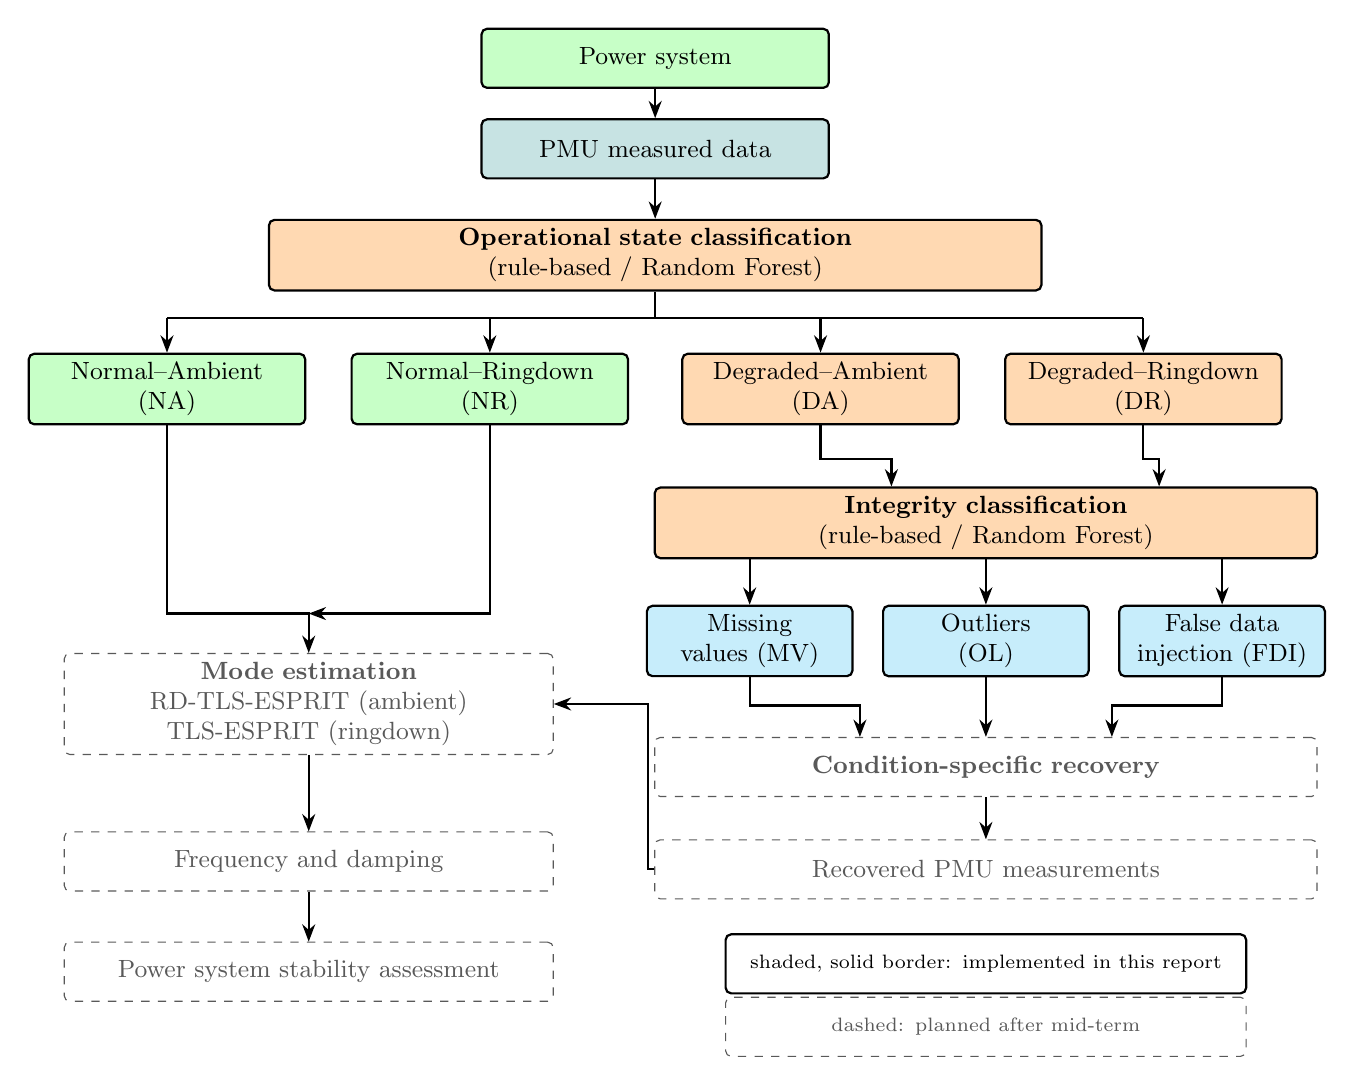
\begin{tikzpicture}[
  box/.style={draw, rounded corners=2pt, minimum height=7.5mm, align=center, font=\small, inner sep=3pt},
  done/.style={box, thick, fill=#1},
  todo/.style={box, dashed, gray!70!black, fill=white},
  arr/.style={-{Stealth[length=2.2mm]}, thick}]
\node[done=green!22, text width=4.2cm] (ps) at (0,0) {Power system};
\node[done=teal!22, text width=4.2cm] (pmu) at (0,-1.15) {PMU measured data};
\node[done=orange!30, text width=9.6cm] (c1) at (0,-2.5) {\textbf{Operational state classification}\\ (rule-based / Random Forest)};
\node[done=green!22, text width=3.3cm] (na) at (-6.2,-4.2) {Normal--Ambient\\(NA)};
\node[done=green!22, text width=3.3cm] (nr) at (-2.1,-4.2) {Normal--Ringdown\\(NR)};
\node[done=orange!30, text width=3.3cm] (da) at (2.1,-4.2) {Degraded--Ambient\\(DA)};
\node[done=orange!30, text width=3.3cm] (dr) at (6.2,-4.2) {Degraded--Ringdown\\(DR)};
\node[done=orange!30, text width=8.2cm] (c2) at (4.2,-5.9) {\textbf{Integrity classification}\\ (rule-based / Random Forest)};
\node[done=cyan!22, text width=2.4cm] (mv) at (1.2,-7.4) {Missing\\values (MV)};
\node[done=cyan!22, text width=2.4cm] (ol) at (4.2,-7.4) {Outliers\\(OL)};
\node[done=cyan!22, text width=2.4cm] (fdi) at (7.2,-7.4) {False data\\injection (FDI)};
\node[todo, text width=8.2cm] (rec) at (4.2,-9.0) {\textbf{Condition-specific recovery}};
\node[todo, text width=8.2cm] (rm) at (4.2,-10.3) {Recovered PMU measurements};
\node[todo, text width=6.0cm] (me) at (-4.4,-8.2) {\textbf{Mode estimation}\\ RD-TLS-ESPRIT (ambient)\\ TLS-ESPRIT (ringdown)};
\node[todo, text width=6.0cm] (fd) at (-4.4,-10.2) {Frequency and damping};
\node[todo, text width=6.0cm] (ss) at (-4.4,-11.6) {Power system stability assessment};
\draw[arr] (ps) -- (pmu); \draw[arr] (pmu) -- (c1);
\coordinate (bus) at (0,-3.3);
\draw[thick] (c1.south) -- (bus);
\draw[thick] (-6.2,-3.3) -- (6.2,-3.3);
\foreach \n in {na,nr,da,dr} \draw[arr] (\n.north |- bus) -- (\n.north);
\draw[arr] (da.south) |- ($(c2.north)+(-1.2,0.35)$) -- ($(c2.north)+(-1.2,0)$);
\draw[arr] (dr.south) |- ($(c2.north)+(2.2,0.35)$) -- ($(c2.north)+(2.2,0)$);
\draw[arr] (c2.south -| mv.north) -- (mv.north);
\draw[arr] (c2.south -| ol.north) -- (ol.north);
\draw[arr] (c2.south -| fdi.north) -- (fdi.north);
\draw[arr] (mv.south) |- ($(rec.north)+(-1.6,0.4)$) -- ($(rec.north)+(-1.6,0)$);
\draw[arr] (ol.south) -- (rec.north -| ol.south);
\draw[arr] (fdi.south) |- ($(rec.north)+(1.6,0.4)$) -- ($(rec.north)+(1.6,0)$);
\draw[arr] (rec) -- (rm);
\draw[arr] (na.south) |- ($(me.north)+(0,0.5)$) -- (me.north);
\draw[arr] (nr.south) |- ($(me.north)+(0,0.5)$);
\draw[arr] (rm.west) -| ($(me.east)+(1.2,0)$) -- (me.east);
\draw[arr] (me) -- (fd); \draw[arr] (fd) -- (ss);
\node[done=white, text width=6.4cm, font=\scriptsize] at (4.2,-11.5) {shaded, solid border: implemented in this report};
\node[todo, text width=6.4cm, font=\scriptsize] at (4.2,-12.3) {dashed: planned after mid-term};
\end{tikzpicture}}
\caption{Workflow of the project. Shaded blocks are implemented in this report; dashed blocks are planned after the mid-term evaluation.}
\label{fig:workflow}
\end{figure}
\section{Data Description}\label{sec:data}
The input is one power measurement (MW) at 30 samples/s: \Nsamples{} samples (\Tdur\,s), giving \Nseg{} one-second segments, with mean \xmean\,MW and standard deviation \xstd\,MW. It contains four ringdowns, R1--R4, near 605, 903, 2680 and 2800\,s (Fig.~\ref{fig:data}). The record is clean: it has no missing samples and the longest run of identical values is \maxflat{} samples. The degraded classes therefore cannot be tested on it directly, and faults with known positions are injected into a copy (Section~\ref{sec:inject}).

\begin{figure}[!t]
\centering
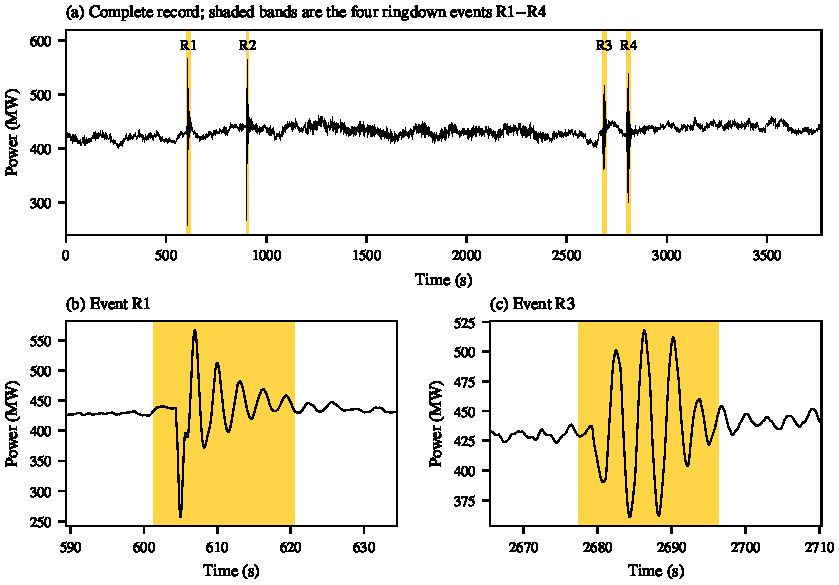
\includegraphics[width=0.72\linewidth]{fig_data.pdf}
\caption{The measured power signal. (a)~Complete record with the four detected ringdowns shaded; (b),(c)~close-ups of R1 and R3.}
\label{fig:data}
\end{figure}

\section{Rule-Based Classification}\label{sec:rules}
Two questions are answered for each one-second segment (30 samples): \emph{is a ringdown present?} and \emph{is the data faulty?}

\subsection{Ringdown Detection}
A ringdown is detected with a short-term/long-term energy ratio (STA/LTA), a detector from seismology \cite{allen1978}. Missing and flat samples are interpolated and a five-point median filter removes short spikes, so that corruption cannot create or hide a ringdown. The result is band-passed (0.2--2\,Hz, zero-phase fourth-order Butterworth) to give $b[k]$, and
\begin{align}
\mathrm{STA}[k] &= \sqrt{\tfrac{1}{W_s}\textstyle\sum_{|j-k|\le W_s/2} b^2[j]},\quad W_s=2f_s,\nonumber\\
\mathrm{LTA}[k] &= \operatorname*{median}_{|j-k|\le W_l/2}\mathrm{STA}[j],\quad W_l=120f_s,\label{eq:lta}\\
r[k] &= \mathrm{STA}[k]/\mathrm{LTA}[k],\label{eq:ratio}
\end{align}
with $f_s=30$\,Hz. A ringdown starts when $r>5$ and $\mathrm{STA}>3$\,MW, ends when $r\le4$ (at most 40\,s), and is accepted only if $b$ crosses zero at least six times, since a level step excites the filter only once or twice.

\subsection{Integrity Checks}
\emph{Missing or stuck data:} a sample is flagged if it is empty or part of a run of at least eight identical values. \emph{Outliers:} with $d^\mp[k]=x[k]-x[k\mp3]$, the spike statistic is
\begin{equation}
e[k]=\begin{cases}\operatorname{sgn}(d^-)\min\{|d^-|,|d^+|\}, & \operatorname{sgn}(d^-)=\operatorname{sgn}(d^+),\\ 0, & \text{otherwise,}\end{cases}\label{eq:spike}
\end{equation}
and a sample is flagged if $|e[k]|>\max\{7\hat\sigma,3\,\text{MW}\}$, where $\hat\sigma$ is a robust noise scale from the median absolute deviation \cite{hampel1974}; inside a ringdown the threshold is raised to half the local swing. \emph{False data injection:} with $m^\mp[k]$ the medians of the 2\,s before and after $k$, the step statistic is
\begin{equation}
S[k]=|m^+[k]-m^-[k]|,\label{eq:step}
\end{equation}
and a step is declared where $S>5\sigma_S$, $\sigma_S=1.4826\operatorname{median}(S)$. An up-step followed within 120\,s by a down-step of similar size marks the whole interval as an offset block.

\subsection{Combining the Checks}
A segment is \emph{ringdown} if more than half of its samples lie in a detected ringdown, and \emph{degraded} if any sample is flagged. With $\ell=\mathbf{1}[\text{ringdown}]+2\cdot\mathbf{1}[\text{degraded}]$,
\begin{equation}
\ell=0\to\text{NA},\ \ell=1\to\text{NR},\ \ell=2\to\text{DA},\ \ell=3\to\text{DR}.\label{eq:label}
\end{equation}
A degraded segment receives the class of the check that flagged it, with priority MV $>$ FDI $>$ OL.

\section{Fault Injection and Validation Data}\label{sec:inject}
Faults are added to a copy $y[k]$ of the clean record $x[k]$, which is never modified, so the type and position of every fault are known. Outliers add an amplitude to one or two samples; missing values are an empty gap, a zero-filled dropout or a frozen value; FDI adds a constant offset $\Delta$ over an interval.

A \emph{hand-placed set} of 17 faults (11 outliers, 3 missing-value blocks, 3 offsets) was placed at chosen times, two of the spikes inside ringdowns. For the Random Forest, \emph{random scenarios} are generated, each with five synthetic ringdowns
\begin{equation}
y[k]=x[k]+A\,e^{-\sigma\tau}\sin(2\pi f\tau),\quad \tau=t[k]-t_0,\label{eq:ringdown}
\end{equation}
$A\sim\mathcal{U}(30,160)$\,MW, $f\sim\mathcal{U}(0.3,1.2)$\,Hz, $\sigma\sim\mathcal{U}(0.1,0.3)\,\mathrm{s}^{-1}$, plus 25 spikes, 5 gaps, 4 zero-filled dropouts, 4 frozen blocks and 8 offsets. Training uses only $t<1850$\,s and testing only $t\ge1950$\,s with different seeds. Scores are per-segment state accuracy and recall, injected faults typed correctly within $\pm1$\,s, and false-alarm segments (degraded segments with no true fault within $\pm1$\,s).

\section{Random Forest Classification}\label{sec:rf}
A Random Forest combines many decision trees, each trained on a random resample and random features, by voting \cite{breiman2001}; it needs no feature scaling and trains in seconds. The scikit-learn implementation is used \cite{pedregosa2011}. Each segment is described by \nFeat{} numbers: 16 measures computed in the segment (missing and zero fraction, longest flat run, spike statistic of Eq.~\eqref{eq:spike}, STA/LTA ratio of Eq.~\eqref{eq:ratio}, zero crossings, level deviation from the surrounding 60\,s and 120\,s, and step statistic of Eq.~\eqref{eq:step}), plus nine of them repeated for neighbouring segments at $\pm1$, $\pm2$ and $\pm4$\,s. They are continuous measures rather than decisions, so the forest learns the boundaries.

Two forests mirror the two classification blocks. \emph{Forest~A} predicts the state (NA, NR, DA, DR); \emph{Forest~B} predicts MV, OL or FDI and is applied only to segments that Forest~A labels DA or DR. Each has 300 trees, at least two samples per leaf and balanced class weights. Six random scenarios are used for training (\trainRows{} segments: \trainNA{} NA, \trainNR{} NR, \trainDA{} DA, \trainDR{} DR).

\section{Results}\label{sec:results}
\subsection{Real Record}
The rules label \rulesRealNA{} segments NA and \rulesRealNR{} NR; the forest gives \rfRealNA{} NA and \rfRealNR{} NR. Neither finds a degraded segment, so there is no false alarm, and they agree on \realAgree\,\% of segments; the \realDiffSeg{} differing segments are ringdown boundaries within \diffMaxDist{} s of a window edge.

\subsection{Hand-Placed Faults}
Fig.~\ref{fig:states_hp} shows the state classification (green: ambient clean, yellow: ringdown clean, brown: ambient corrupted, red: ringdown corrupted), and Fig.~\ref{fig:types_hp} the integrity class assigned to each fault against the ground truth. Both classifiers type all \hpEvents{} faults correctly, with \hpFAru{} false-alarm segments for the rules and \hpFArf{} for the forest. The rules mark \hpExtraRu{} extra segments around offset blocks, because their step test uses two-second windows widened by one second; the forest marks \hpExtraRf{}. Both give DR for the two spikes inside ringdowns.

\begin{figure}[!t]
\centering
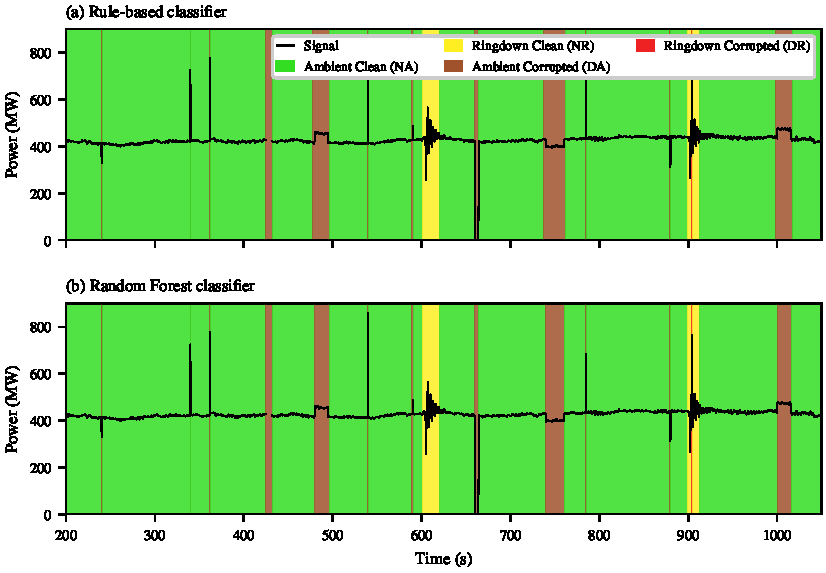
\includegraphics[width=0.74\linewidth]{fig_states_hp.pdf}
\caption{State classification with the 17 hand-placed faults (200--1050\,s): (a)~rule-based, (b)~Random Forest.}
\label{fig:states_hp}
\end{figure}

\begin{figure}[!t]
\centering
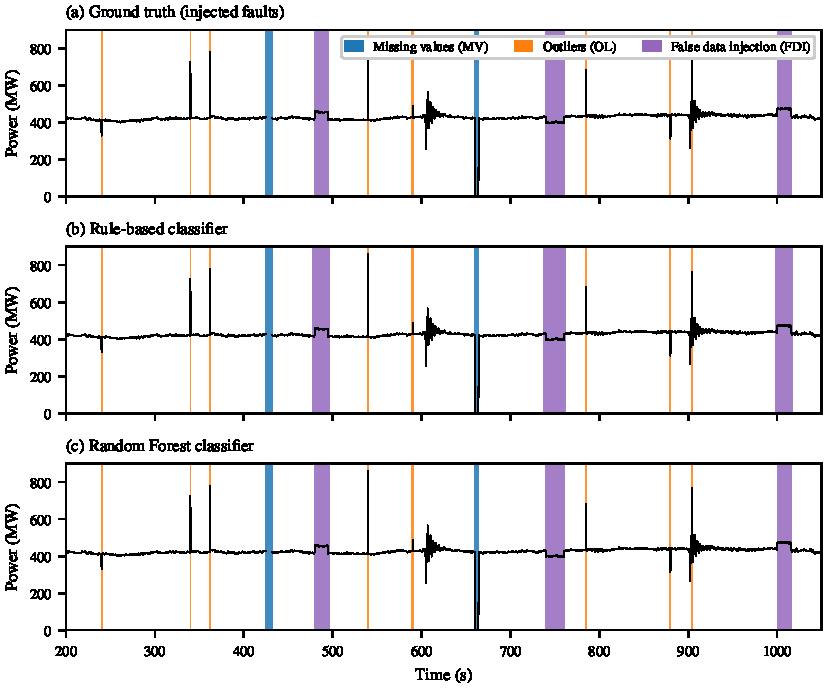
\includegraphics[width=0.72\linewidth]{fig_types_hp.pdf}
\caption{Integrity classes of the hand-placed faults: (a)~ground truth, (b)~rule-based, (c)~Random Forest. Blue: MV; orange: OL; purple: FDI.}
\label{fig:types_hp}
\end{figure}

\subsection{Random Hold-Out Scenarios}
Five random scenarios from $t\ge1950$\,s (\hoEvents{} faults, \hoN{} segments), unseen in training, give Table~\ref{tab:scores}. The forest has the higher accuracy (\hoRfAcc\,\% against \hoRuAcc\,\%), the higher ringdown recall (\hoRfNR\,\% against \hoRuNR\,\%) and far fewer false alarms (\hoFARf{} against \hoFARu{} segments). Both are weakest on DR, with recalls of \hoRfDR\,\% and \hoRuDR\,\%.

\begin{table}[!t]
\centering
\small
\begin{tabular}{@{}lrr@{}}
\toprule
Measure & Rules & Random Forest \\
\midrule
State accuracy (\%) & 92.3 & 98.3 \\
Recall of NA (\%) & 94.3 & 99.5 \\
Recall of NR (\%) & 70.5 & 92.1 \\
Recall of DA (\%) & 91.6 & 96.8 \\
Recall of DR (\%) & 43.7 & 41.4 \\
\midrule
MV events typed correctly & 64 of 72 & 69 of 72 \\
OL events typed correctly & 131 of 140 & 137 of 140 \\
FDI events typed correctly & 38 of 40 & 40 of 40 \\
False-alarm segments & 333 & 4 \\
\bottomrule
\end{tabular}

\caption{Scores on the five hold-out scenarios.}
\label{tab:scores}
\end{table}

\section{Discussion and Limitations}
On the real record the methods are practically equivalent, on hand-placed faults both are correct, and on random scenarios the forest is more accurate. The evidence has limits. (i)~All fault results are synthetic, and real PMU faults may differ. (ii)~The forest was trained on the same generator that produced the hold-out scenarios, whereas the rule thresholds were tuned by hand, so the comparison favours the forest; the real-record comparison is the fairer one. (iii)~The real ringdown windows come from the rule-based detector, with no independent label. (iv)~DR is weakly detected, as few examples combine a ringdown with a fault. (v)~FDI is limited to constant offsets, and (vi)~one record was used.

\section{Conclusion and Future Work}\label{sec:future}
A rule-based and a Random Forest classifier were implemented for the operational states NA, NR, DA, DR and the integrity classes MV, OL, FDI. Both label the real record as clean and agree on \realAgree\,\% of segments; on injected faults the forest is the more accurate with fewer false alarms. After the mid-term evaluation the plan is: condition-specific recovery of degraded data (the recovery error can be measured exactly since the original is clean); mode estimation with TLS-ESPRIT and RD-TLS-ESPRIT \cite{roy1989}, checked on the synthetic ringdowns of Eq.~\eqref{eq:ringdown}; stability assessment from the damping ratios.

\addcontentsline{toc}{section}{\protect\numberline{}References}
\begin{thebibliography}{99}\small\linespread{1.1}\selectfont
\bibitem{kundur2004} P. Kundur \emph{et al.}, ``Definition and classification of power system stability,'' \emph{IEEE Trans. Power Syst.}, vol. 19, no. 3, pp. 1387--1401, Aug. 2004.
\bibitem{liu2009} Y. Liu, P. Ning, and M. K. Reiter, ``False data injection attacks against state estimation in electric power grids,'' in \emph{Proc. 16th ACM Conf. Comput. Commun. Secur. (CCS)}, Chicago, IL, USA, Nov. 2009, pp. 21--32.
\bibitem{breiman2001} L. Breiman, ``Random forests,'' \emph{Mach. Learn.}, vol. 45, no. 1, pp. 5--32, Oct. 2001.
\bibitem{roy1989} R. Roy and T. Kailath, ``ESPRIT---Estimation of signal parameters via rotational invariance techniques,'' \emph{IEEE Trans. Acoust., Speech, Signal Process.}, vol. 37, no. 7, pp. 984--995, Jul. 1989.
\bibitem{allen1978} R. V. Allen, ``Automatic earthquake recognition and timing from single traces,'' \emph{Bull. Seismol. Soc. Amer.}, vol. 68, no. 5, pp. 1521--1532, Oct. 1978.
\bibitem{hampel1974} F. R. Hampel, ``The influence curve and its role in robust estimation,'' \emph{J. Amer. Statist. Assoc.}, vol. 69, no. 346, pp. 383--393, Jun. 1974.
\bibitem{pedregosa2011} F. Pedregosa \emph{et al.}, ``Scikit-learn: Machine learning in Python,'' \emph{J. Mach. Learn. Res.}, vol. 12, pp. 2825--2830, Oct. 2011.
\end{thebibliography}
\end{document}
